\documentclass[a4paper,10pt]{article}
\usepackage[utf8]{inputenc}
\usepackage{geometry} %自定义布局
\usepackage{multicol} %双栏
\usepackage{graphicx} %图像
\usepackage{amsmath} % 数学单位等等
\usepackage[runin]{abstract} %摘要修改
\usepackage{booktabs}%三线格
\usepackage{float}%浮点
\usepackage{cite}%引用
\geometry{a4paper,left=1.6cm,right=1.6cm,top=2cm,bottom=2cm}
\graphicspath{{picture/},{pics/}}
%opening
\title{Genotyping and Population Genetic Analysis of TPA-25 and VWA Microsatellites Through PCR-base Screening, Gel Electrophoresis and Statistical Method}
\author{Mingbai Zeng , Kangyao Ma , Haozhan Yuan , Yimeng Yuan}
\date{}

\begin{document}

\maketitle

\setlength{\absleftindent}{0pt}
\setlength{\absrightindent}{0pt}
\setlength{\abstitleskip}{-1.5em}
\abslabeldelim{:}
\renewcommand{\absnamepos}{flushleft}
\begin{abstract}
This study investigates the genotyping and population genetics of the TPA-25 and VWA microsatellite loci through a PCR-based screening approach, gel electrophoresis and statistical analysis. The objective of the first experiment was to analyze the TPA-25 genotype frequencies in a class population, ascertain whether these frequencies are in Hardy-Weinberg equilibrium. The second experiment aimed to determine the range of fragment sizes and distribution at the VWA locus, to assess genetic diversity and evaluate its utility as a marker for individual identification. DNA was extracted from cheek cells, and PCR amplified the loci, with agarose and polyacrylamide gel electrophoresis being utilized to separate and visualize the PCR products. Gel images were analyzed to estimate allele and genotype frequencies, while Chi-square tests were applied to compare observed and expected frequencies as per the Hardy-Weinberg Principle. Suggestions to enhance the accuracy of the experiments included the use of fluorescent capillary electrophoresis and improving primer specificity. The accuracy of repeat estimation was considered, with strategies proposed to refine the precision of these estimations in further iterations of the research.

\end{abstract}
\hrule

\begin{multicols}{2}
\section{Introduction}

Alu family members which belong to the short-interspersed elements (SINEs) are predominantly distributed in the human genome \cite{harris2017unbiased}. By the retro-transposition machinery, the Alu elements have accumulated about 1.1 million copies over the past 65 million years in the human genome and it is estimated to comprise 11\% of the total genome \cite{venter2001sequence}. TPA-25, a recently found dimorphic Alu insertion element which located in the intron of the human genome has both homozygote and heterozygote individuals \cite{perna1992alu}.According to the previous research, the results of the PCR-base (polymerase chain reaction) screen for TPA-25 using oligonucleotide primers showed 400 bp for the presence of the TPA-25 insertion and 100 bp for the absence \cite{batzer1991amplification}.

Microsatellite sequences, also known as short tandem repeats (STRs), are omnipresent repeating sequences in the human genome and have extremely abundant mutational mechanisms \cite{wiegand2000microsatellite}. According to Eckert and Hile , microsatellites are mostly produced by the slippage of DNA polymerases \cite{eckert2009every}. The microsatellite has a higher mutation rate than the base-pair substitutions and its frequency is 10- to 100-fold higher than the frameshift in coding sequence. The property of the microsatellite mutation rate makes it competent for studying evolution over a short time span. On the other hand, polymorphic STR loci are extensively used in the forensic and individual identification area \cite{gavale2024rare}. And according to Gavale, the inheritance pattern of STRs follows the general Mendelian pattern. VWA locus which belongs to the STRs is the target of this experiment. It has a size range from 130 to 170 bps with the repeat units TCTA(TCTG)3-4(TCTA)n.

Experiment 1 aims to perform the PCR-base screening and agarose gel electrophoresis for the whole class to gather statistical data about the genotype frequencies of the TPA-25 in the class population and compare the data with the expected frequencies to elucidate whether the TPA-25 element follows the Hardy-Weinberg Principle in the class population. Experiment 2 aims to use PCR and polyacrylamide gel electrophorese to indicate the length range and the distribution of the different fragment sizes of the VWA locus in the class population and also to justify the reliability of using the VWA locus as the indicator for individual identification.



\section{Material and method}
\subsection{DNA extraction}
To extract DNA, cheek cells were collected using a sterile mouth swab and suspended in a saline solution. The swab was immersed in a tube with 1000 \textmu l of 0.9\% (w/v) NaCl solution and vortexed for 15 seconds to dislodge the cells. The cells were centrifuged at 11,000 rpm for 10 minutes, then discarding the saline solution. After centrifugation, the supernatant was discarded and the cell pellet was resuspended in 500 \textmu l of 10\% Chelex solution. The sample was then vortexed and incubated at 100°C for 10 minutes with repeated agitating. After heat block, the sample was chilled on ice for 1-2 minutes before being centrifuged at 13,000 rpm for 30 seconds. 200 \textmu l of the clear supernatant with the DNA was transferred to a fresh tube.


\subsection{Polymerase chain reaction (PCR)}
The TPA-25 genotype was determined using PCR with specific primers flanking the TPA-25 Alu insertion site. The reaction system contained DNA template, PCR buffer, primers, dNTPs, Q-solution, and Taq polymerase. Reactions were subjected to 30 cycles consisting of an initial denaturation at 94°C for 30 sec, followed by 30 cycles of denaturation, annealing at 58°C for 30 sec, and extension at 72°C  for 45 sec with a final hold at 4 degrees Celsius.


\subsection{Gel electrophoresis and gel imaging }
Agarose gel electrophoresis was used to separate the PCR products. A 2\% agarose gel which was stained with GelRed was prepared, loaded with the PCR products and a molecular marker, and run at 100 volts for 45 minutes. Finally, the gel was visualized under UV light to determine the presence or absence of the TPA-25 insertion and to analyze the micro-satellite alleles. The gel was produced in 1X TAE buffer with GelRed added at a 1:10,000 dilution. Each well was loaded with 20 \textmu l of PCR product mixed with 4 \textmu l of 6X loading dye and the gel was run for 45 minutes at 100 volts. The genotyping results were then used to estimate allele frequencies within the class population and to assess the genetic diversity and structure using the Hardy-Weinberg Principle. Polyacrylamide gel was used for imaging the PCR result for the VWA locus.


\subsection{Statistical analysis}
Analysis was undertaken using the following statistical packages: GENEPOP software was used to assess Hardy-Weinberg equilibrium (HWE); The frequency of each allele for each locus tested was calculated by Power Marker\cite{liu2005powermarker}. Polymorphic information content (PIC), observed heterozygosity (Ho), expected heterozygosity (He) were performed with Power Marker.


\begin{center}
\textbf{Table 1.Materials needed for this experiment}
\vspace{0pt}
\begin{tabular}{cc}

\toprule [1.5pt]
\textbf{DNA Extraction}&\textbf{Dose}\\
\hline
Sterile mouth swabs&/\\
Bijou tubes&/\\
1.5 mL screw-top-tubes&/\\
0.5 mL microcentrifuge tubes&/\\
0.9\% (w/v) NaCl&1000\textmu L\\
10\% Chelex&500\textmu L\\
Ice& / \\
\hline
\textbf{PCR}&\\
\hline
DNA or H2O for control&5.0 \textmu L\\
10X PCR buffer (with dye)&2.5\textmu L\\
TPA-25 Forward primers&1.25\textmu L(10mM,20X)\\
TPA-25 Reverse primers&1.25\textmu L(10mM,20X)\\
dNTP mix&0.5\textmu L(10mM,50X)\\
Q-solution&5.0\textmu L(5X)\\
ddH2O&8.5\textmu L\\
Taq polymerase&1.0\textmu L\\
\hline
\textbf{Gel electrophoresis}&\\
\hline
2\% agarose in 1X TAE&100mL\\
5\% polyacrylamide in 5X TBE&/\\
Gel Red&1:10000\\
Loading buffer&6X\\
Molecular marker&/\\
\bottomrule [1.5pt]
\end{tabular}
\end{center}


%\end{multicols}


%\begin{figure}[htbp]
%\centering
%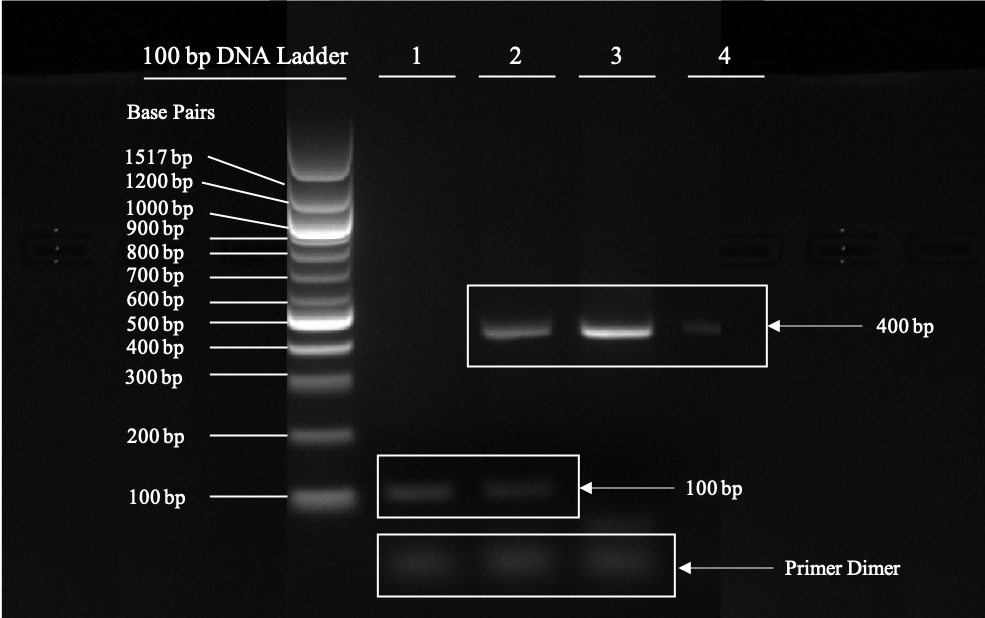
\includegraphics{tpa25.png}
%\caption{bionux}
%\end{figure}

%\begin{multicols}{2}

\section{Results and analysis}
\subsection{TPA-25}
The agarose gel image of the G24 group (Figure 1) which is used as a representation, demonstrates the presence of the TPA-25 dimorphic insertion and different genotypes. Sample 1 which has only one band at around 100 bp is a homozygote (-,-) which is absent with the TPA-25 element. Sample 2 has two bands in which the individual is a heterozygote (+,-) with one chromosome having the TPA-25 element and the other absence. Samples 3 and 4 are both homozygote (+,+) with TPA-25 in both sets of chromosomes which generate only one band at around 400 bp. The genotype data of the whole class population were collected and summarized in Table 1. The total counts of homozygous samples, heterozygous samples (+/-), and homozygote samples without the TPA-25 insertion (-/-) were 30, 19, and 44, respectively.

\begin{figure}[H]
\centering
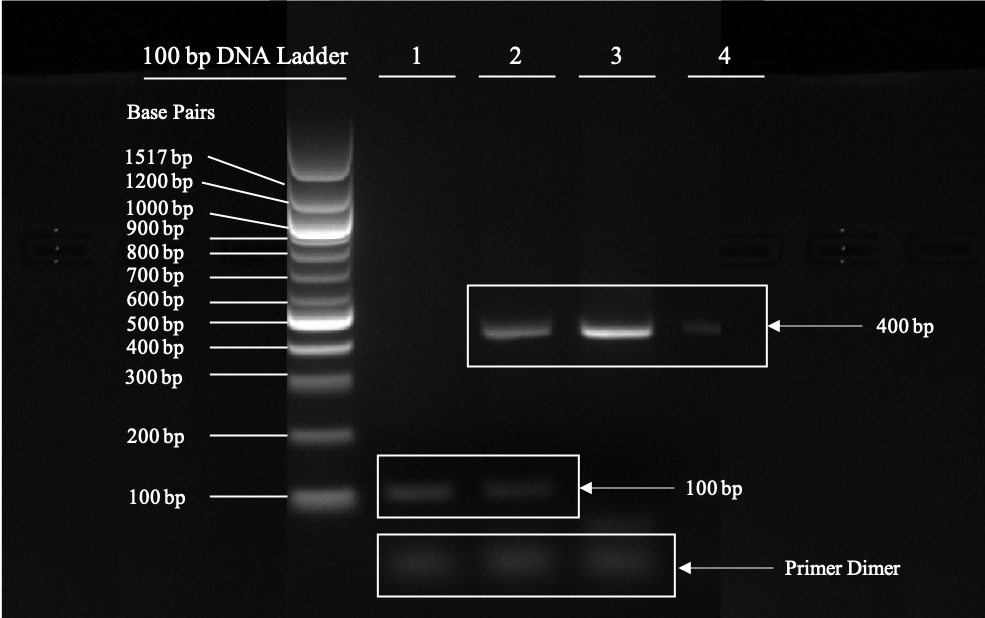
\includegraphics[width=0.48\textwidth]{tpa25.png}
\caption{G24 Agarose gel electrophoresis image of TPA-25 Alu insertion element. Land 1 homozygote (-,-) has only one band at 100 bp. Lands 3 and 4 homozygotes (+,+) have only one band at 400 bp. Land 2 heterozygote (+,-) has bands at both 100 bp and 400 bp. The bands at the bottom are primer dimers.} \label{fig1}
\end{figure}


\begin{center}
\textbf{Table 2.Genotype number, actual ratio and expected ratio of TPA-25 experimental statistics}
\vspace{0pt}
\begin{tabular}{cccc}

\toprule [1.5pt]
&100/100 -/-&400/100 +/-&400/400 +/+\\
\hline
Number&19&44&30\\
Observed&0.204&0.473&0.323\\
Expected&0.198&0.493&0.308\\
\bottomrule [1.5pt]
\end{tabular}
\end{center}



To verify whether the TPA-25 Alu insertion element follows the Hardy-Weinberg genetic equilibrium and to determine whether the observing and expected frequencies have a significant deviation a statistical analysis of the genotype frequency was conducted with a chi-square test(formula 1). The null hypothesis of the test is that the observed frequencies have no significant deviance from the expected frequencies. The degree of freedom of the chi-square test can be calculated with the number of categories minus one. TPA-25 has two alleles so the degree of freedom is 1. If the confidence level is set as 0.05 with 95\% confidence, the critical value of the chi-square testing has a significance level of 3.841 known the df is 1. The chi-square statistic of the alleles frequency is 0.161 which is significantly less than the 3.841, critical value. Consequently, the null hypothesis that the observed frequencies have no significant difference from the expected frequencies cannot be rejected at a 0.05 significance level. So it can be concluded that the TPA-25 follows the Hardy-Weinberg genetic equilibrium.The following part is the calculation process


\setlength{\parindent}{0pt}Allele frequency calculation:
$$\mathrm{P}_{(+)}=\mathrm{P}_{(+/+)}+\mathrm{P}_{(+/-)}\div2=0.555$$
$$\mathrm{P}_{(-)}=\mathrm{P}_{(-/-)}+\mathrm{P}_{(+/-)}\div2=0.445$$
Expected genotype frequency calculation:
$$\mathrm{P}_{exp(+/+)}=\mathrm{P}_{(+)}^2=0.308$$
$$\mathrm{P}_{exp(+/-)}=\mathrm{P}_{(+)} \times \mathrm{P}_{(-)} \times 2 =0.493$$
$$\mathrm{P}_{exp(-/-)}=\mathrm{P}_{(-)}^2=0.198$$
Chi-square results:
\begin{equation}\chi^2=\sum\frac{(\text{observed}-\exp)^2}{\exp}=0.161\end{equation}


\subsection{vWA microsatellite}

The Polyacrylamide gel image of the G24 group (Figure 2) is used as a representation. As Figure 2 illustrates, land 2 has a fragment the size of around 158 bp. Land 3 and 4 have bands of around 154 bp and Land 1 have a fragment size of around 150 bp. The 4 samples are both homozygotes. The fragment size and the frequency of the whole class population are collected and summarized in Table 2. According to previous research, the VWA microsatellite length ranges from 126 to 170 bp, so the fragment size of the experiment results were all estimated by the naked-eye observation and fit in the proper range.

\begin{figure}[H]
\centering
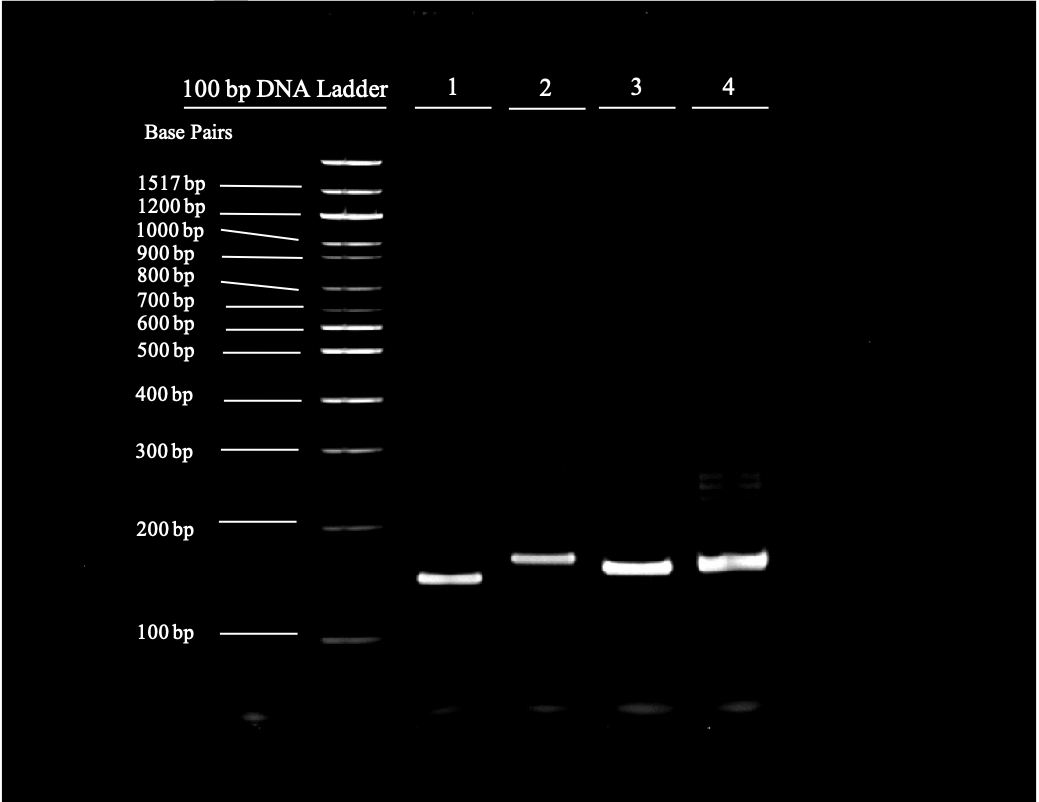
\includegraphics[width=0.48\textwidth]{vwa1.png}
\caption{G24 Polyacrylamide gel electrophoresis image of VWA microsatellite. Land 2 has a fragment size of around 158 bp. Land 3 and 4 have the bands at around 154 bp. Land 1have a fragment size of around 150 bp. The 4 samples are homozygotes.} \label{fig2}
\end{figure}


\begin{center}
\textbf{Table 3.Distribution of vWA genotypes}
\vspace{0pt}
\begin{tabular}{c|ccccccccc}
\toprule [1.5pt]
Allele&14&15&16&17&18&19&20&21&22\\
\hline
12&&&1&1&&&&\\
13\\
14&1&&1&5&1\\
15&&3&&1&1&3&2&1&\\
16&&&6&&3&2&4&1\\
17&&&&6&&3&2&2\\
18&&&&&14&&1&&1\\
19&&&&&&7&&1&\\
20&&&&&&&4&&3\\
21&&&&&&&&3&1\\
22&&&&&&&&&1\\
\bottomrule
\end{tabular}
\end{center}


Summarizing the data, it can be noticed that most of the samples of the class population were generated in one or two bands due to the diploidy of the cheek cells. The VWA microsatellite on chromosomes of the cells is inherited following the general Mendelian pattern. Normally, the homozygote offspring that inherit alleles which have the same length of microsatellite from the parent will generate one band and the heterozygote offspring that inherit different lengths of allele will generate two bands. The microsatellites have a high mutation rate and it is easy for DNA polymerases to slippage due to their repeating property which led to variability in genotype and caused a higher frequency of individuals that generated two bands in the experiment. However, the experiment’s results show that some individuals’ DNA samples generate more than two bands with three or four bands specifically. The reason for this phenomenon might be caused by microvariants, slippage mutation in early somatic cell development, primer binding site mutations and chimerism \cite{gavale2024rare}.



The gene locus frequency and genotype frequency of the vWA gene are presented in Table 3, with alleles named according to the number of core sequence repeats (n) \cite{van2015forensic}. The vWA gene comprises three regions (V-I to V-III), with variations in repeat numbers in the V-III region being the primary cause of allele diversity. The most prevalent structural type in the human genome is (TCTA)(TCTG)4(TCTA)n \cite{minaguchi2000structural}. Previous studies have shown that the PCR amplification product range of the vWA locus is between 126 and 170 bp (alleles 11-20) \cite{cp1992further}. The vWA gene base data obtained in this study range from 130bp to 170bp, corresponding to repeat numbers of (TCTA) from 12 to 22, based on the most common vWA sequence structure. Population genetic analyses were conducted on the data. Due to the lack of a clear distinction between dominant and recessive traits and the absence of gender influence on the vWA gene, the Minimum Pearson X2 test was used to assess Hardy-Weinberg equilibrium of the vWA data, yielding a P-value of 0.1031 (\textgreater0.05), indicating Hardy-Weinberg equilibrium \cite{harris2017unbiased}. Additionally, the polymorphism information content (PIC) was calculated to be 0.88, with an expected (He) heterozygosity of 0.898 and an observed (Ho) heterozygosity of 0.68 \cite{serrote2020determining}.


\begin{equation}\begin{aligned} \chi^2&=\sum_{i=1}^m\frac{(n_i-nq_i)^2}{nq_i}\\&=\sum_{i=1}^m\frac{n_i^2}{nq_i}-2n+n\\&=\sum_{i=1}^m\frac{n_i^2}{nq_i}-n \end{aligned}\end{equation}

\begin{equation}PIC=1-\sum_{i=1}^np_i^2-\left(\sum_{i=1}^np_j^2\right)^2+\sum_{i=1}^np_i^4\end{equation}

\begin{equation}H_{\exp}=1-p^2-q^2\end{equation}


PIC can be defined as the frequency of polymorphism for a marker in a population, which can be used to indicate the level of polymorphism at a locus within a population\cite{botstein1980construction}. PIC depends on the number of alleles detected and their frequency distribution. The larger the number of alleles and the more equal their frequencies, the higher the PIC. The minimum value approaches 0, while the maximum approaches 1. In forensic identification, PIC can be used as the power of discrimination (PD) to assess whether a locus can be used for individual identification \cite{bhinder2018se33}. In a study on the STR polymorphisms in the Indonesian population, the polymorphism information content (PIC) of 13 loci ranged from 0.642 for TPOX to 0.921 for vWA, all suitable for forensic identification \cite{manela2023dna}. The PIC value of 0.88 obtained for the vWA gene in this experiment is sufficient to demonstrate that the vWA gene in the Chinese population can be used for forensic identification.

Genetic heterozygosity refers to the proportion of individuals in a population that are heterozygous at a given allele locus. The expected heterozygosity is much greater than the observed heterozygosity, indicating that there are fewer heterozygotes in the experimental data than expected. Previous studies have shown that under normal conditions, the He and Ho of the vWA gene are similar and do not show significant discrepancies \cite{foroughmand2014genetic}. The difference between He and Ho is usually due to factors such as inbreeding \cite{aguiar2011updated}, which is less likely to occur in the experimental population. Therefore, the large difference between the actual and expected heterozygosity may be due to erroneous statistics in the results. In the gel image of the experiment, there are two DNA bands in each lane, representing the two alleles of vWA. If there is only one band generated, it indicates a homozygote. Statistical analysis of heterozygosity suggests that many bands may not have completely separated during gel electrophoresis, leading to the inability to correctly identify genotypes with alleles of similar sizes as homozygotes or heterozygotes \cite{yunis2005population}.

Compare the vWA locus allele frequency between the experimental population and different populations, the allele frequency distribution characteristics of vWA locus are different in different populations. The common alleles in the experimental population are vWA18, and the common alleles in Henan Han and Chengdu Han are vWA14 and vWA17. vWA16 has the highest gene frequency among black Americans and Hispanics, and vWA17 has the highest gene frequency among whites and southeastern Hispanics. Highest.

\begin{figure}[H]
\centering
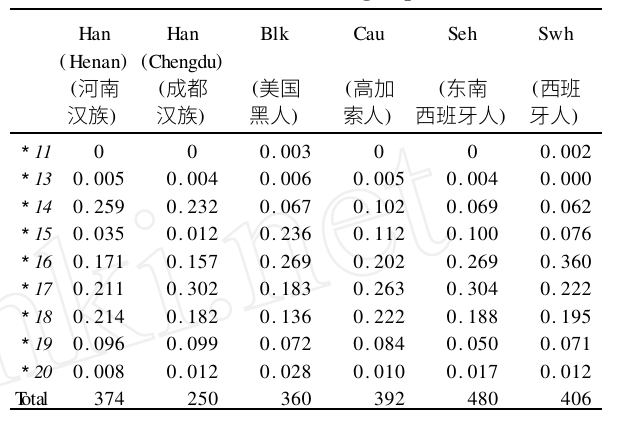
\includegraphics[width=0.5\textwidth]{genel.png}
\caption{Sequence structure of common vWA alleles} \label{fig3}
\end{figure}

\end{multicols}


\begin{center}
\textbf{Table 4.Number and frequency of each allele}
\vspace{0pt}
\begin{tabular}{ccccccccccc}
\toprule [1.5pt]
12&13&14&15&16&17&18&19&20&21&22\\
\hline
2&0&9&14&24&26&35&23&20&12&7\\
0.012&0.000&0.052&0.081&0.140&0.151&0.203&0.134&0.116&0.070&0.040\\
\bottomrule
\end{tabular}
\end{center}



\begin{figure}[H]
\centering
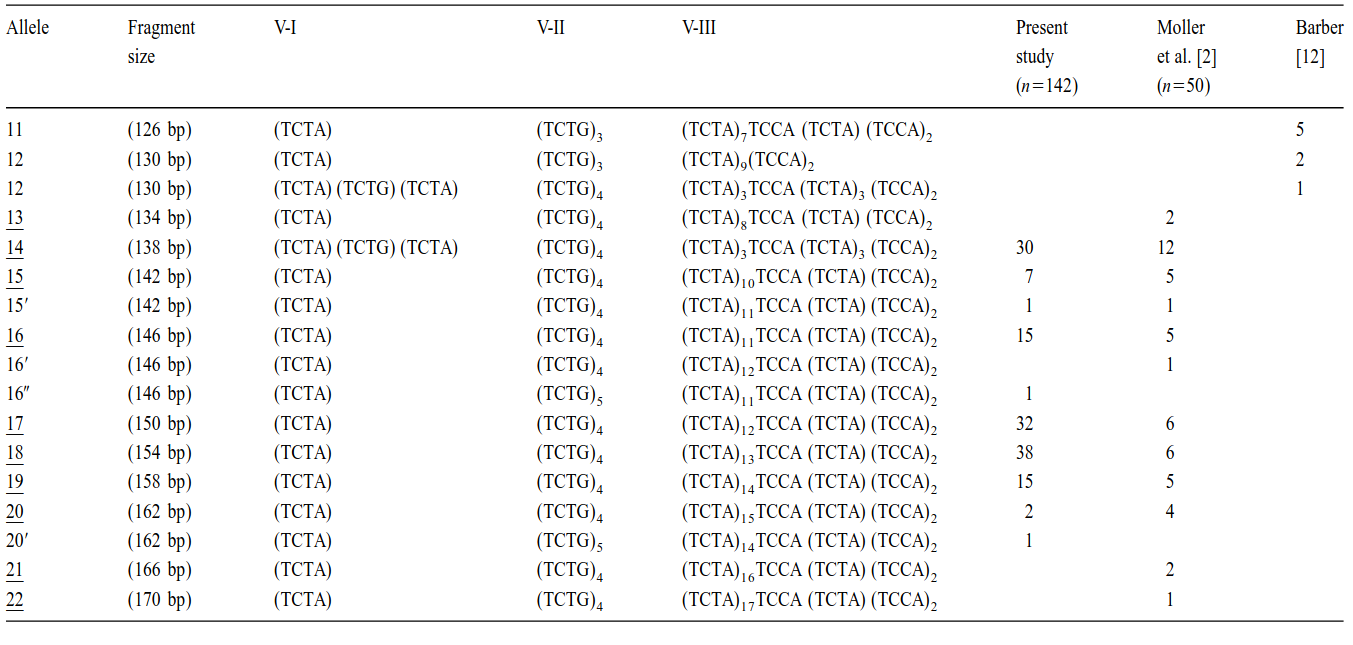
\includegraphics[width=1\textwidth]{vwamay.png}
\caption{Sequence structure of common vWA alleles} \label{fig3}
\end{figure}







\begin{figure}[H]
\centering
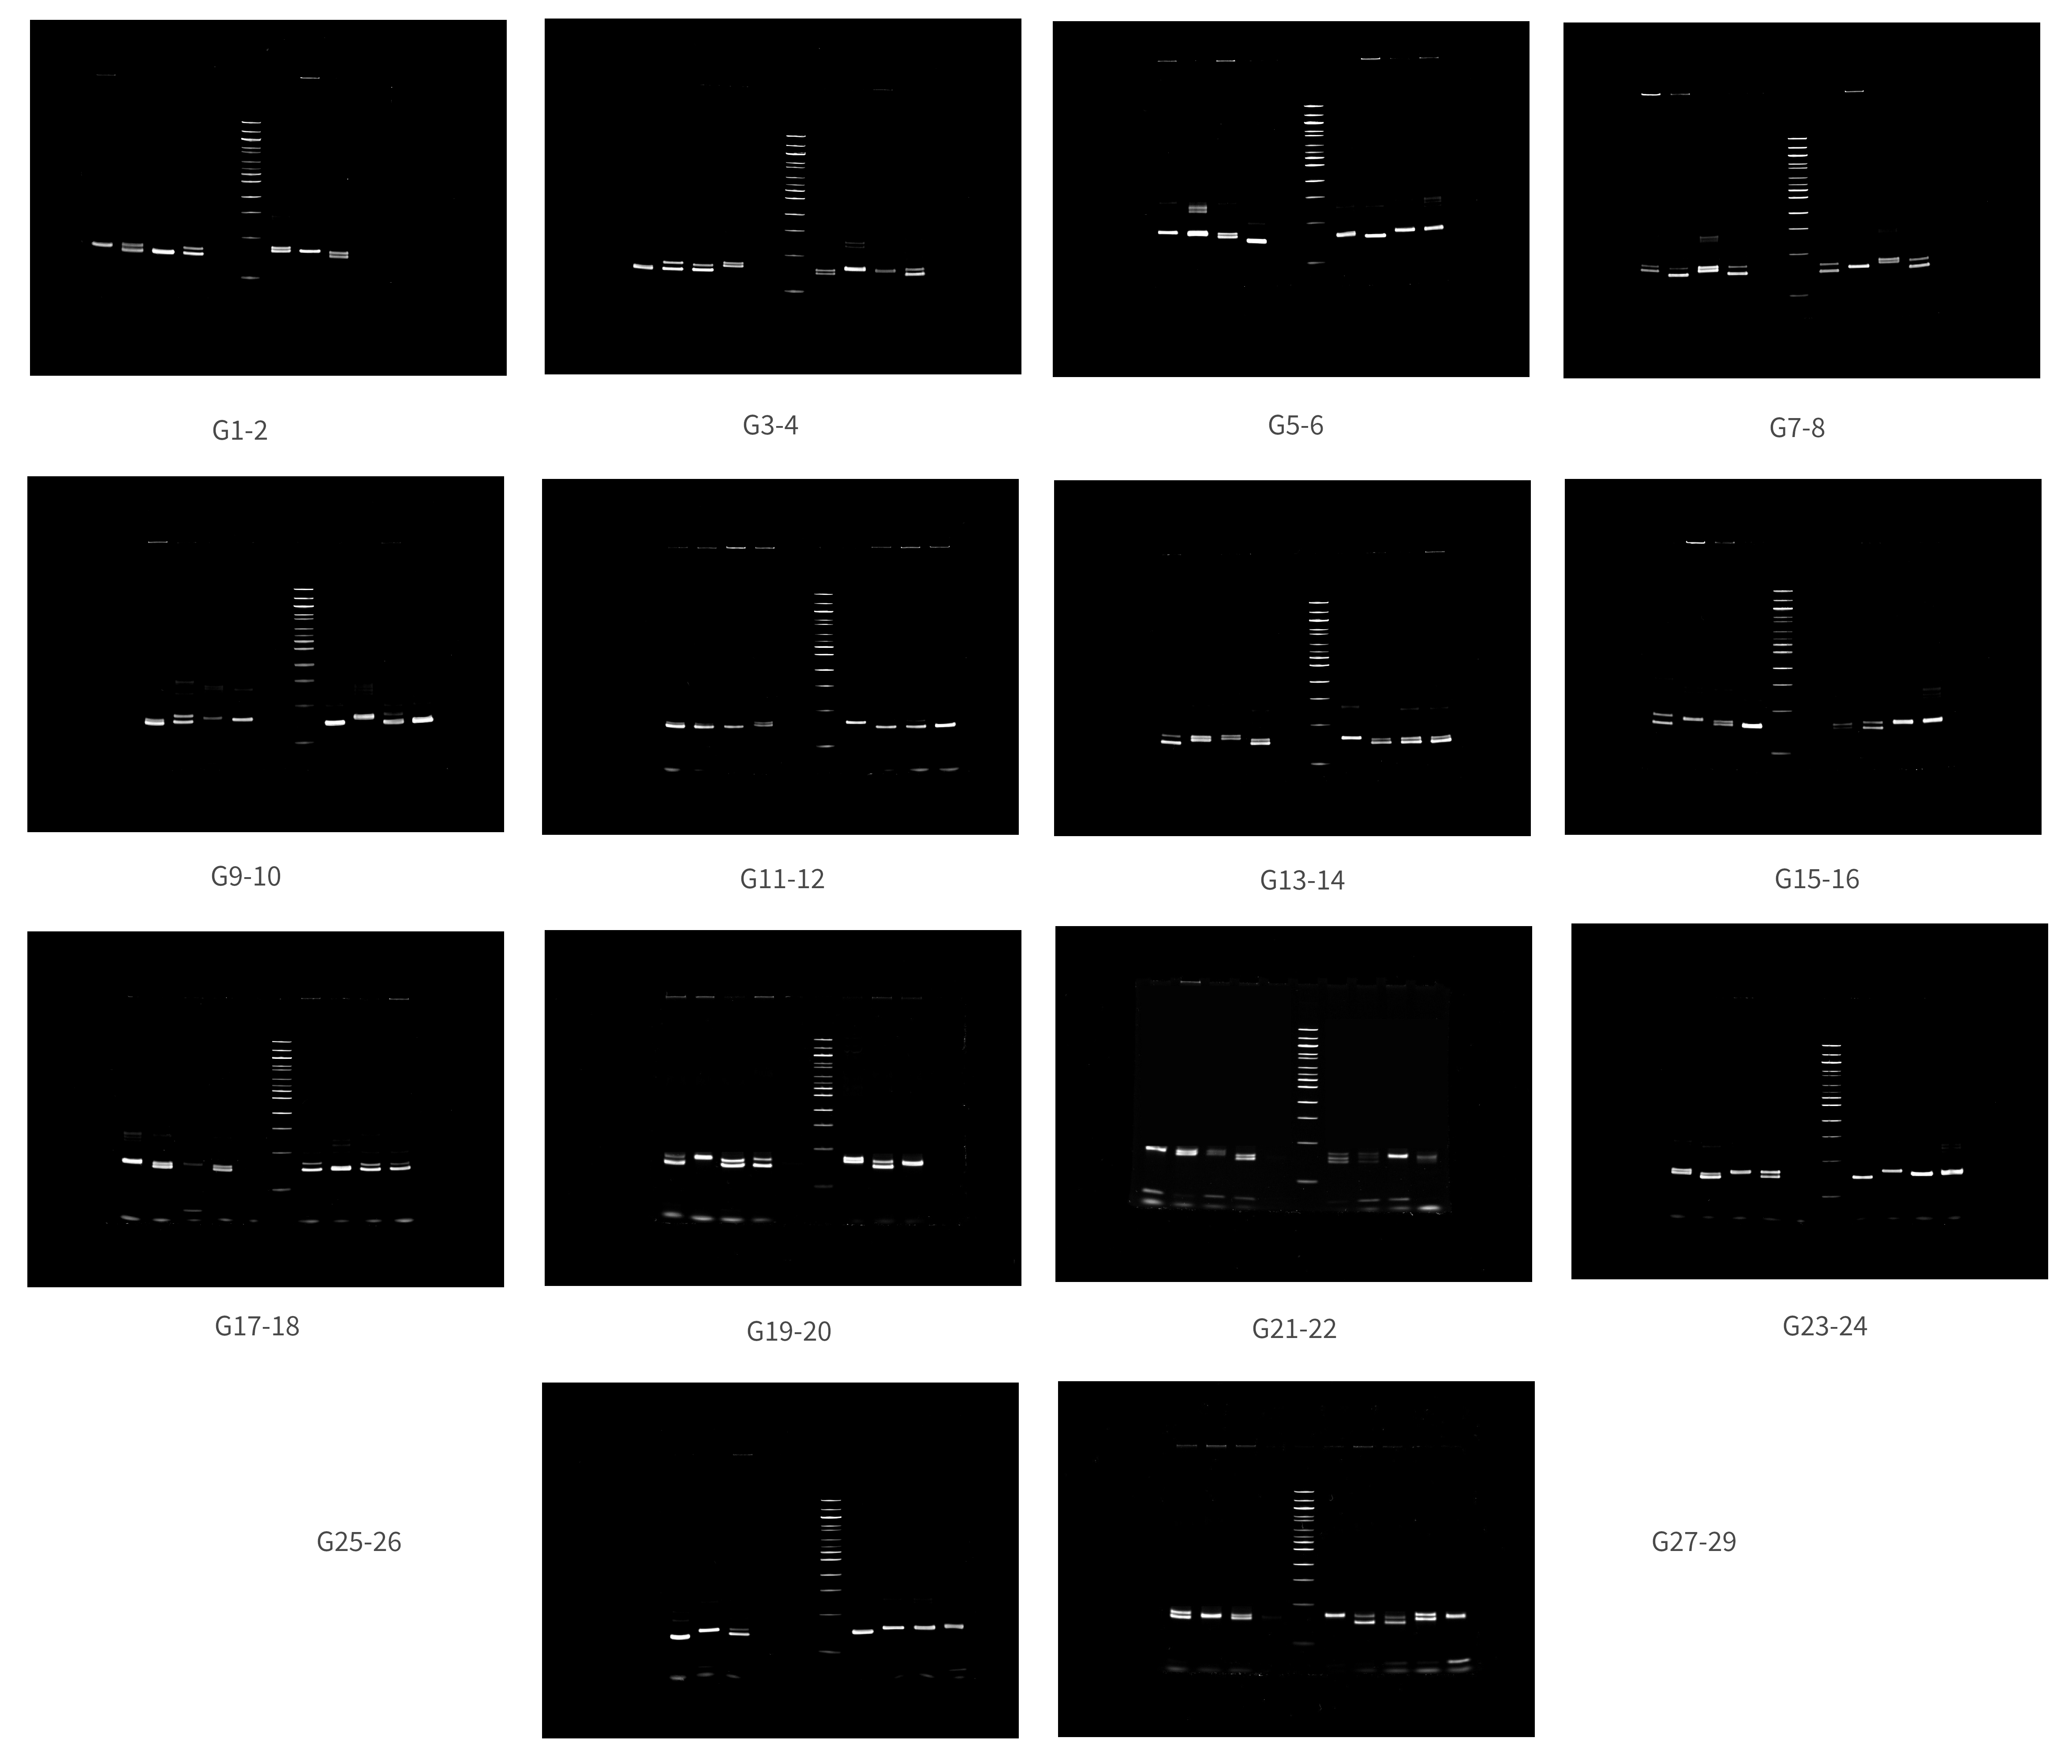
\includegraphics[width=0.9\textwidth]{vwa.png}
\caption{Raw image data of vWA gene} \label{fig3}
\end{figure}



\begin{multicols}{2}
\section{Discussion and conclusion}

According to previous research, the TPA-25 insertion has a frequency range from 13.6\% to 58.0\%. (Perna, et al. 1992) In this experiment, the TPA-25 have a frequency of 55.91\% which is still in the range of the previous research. The deviation of the frequency might result from the population distribution.

There are several experimental procedures and laboratory operations, which might affect the precision and reliability of the experiment result, that need to be refined. For DNA extraction, the swab might not be able to collect enough check cells which might cause the failure of the DNA extraction and consequently fail the experiment. The specificity of the PCR primer needs to be improved to prevent multiple binding or miss-binding which might lead to the wrong amplification of the target fragment and cause the miss-estimation of the fragment length. The gel electrophoresis and gel imaging which are used to illustrate the PCR product size might be imprecise when collecting and processing the data by naked-eye observation. Fluorescent capillary electrophoresis resultant amplicons can be used for result analysis which could provide more precise and quantizable data.

In conclusion, Experiment 1 effectively demonstrates the different genotypes of the TPA-25 element which meet the previous research with three genotypes and justifies that the genotype frequency of the TPA-25 follows the Hardy-Weinberg Principle. The variety and the uniqueness of the vWA microsatellite genotype among individuals had been justified by Experiment 2 and proved that the vWA locus is suitable for use in individual identification.


\bibliographystyle{unsrt}
\bibliography{reference}

\end{multicols}

\end{document}
